\documentclass[12pt, a4paper, openany]{article}

\usepackage[utf8]{inputenc}
\usepackage[T1]{fontenc}
\usepackage[a4paper,left=2cm,right=2cm,top=2cm,bottom=2cm]{geometry}
\usepackage[frenchb]{babel}
\usepackage{libertine}
\usepackage[pdftex]{graphicx}
\usepackage[usenames,dvipsnames,svgnames,table]{xcolor}
\usepackage{soul}
\usepackage{times}
\usepackage{hyperref}

\setlength{\parindent}{0cm}
\setlength{\parskip}{1ex plus 0.5ex minus 0.2ex}

\newcommand{\hsp}{\hspace{20pt}}
\newcommand{\HRule}{\rule{\linewidth}{0.5mm}}

\usepackage{listings}
\usepackage{color}
\usepackage{tabularx,multirow}
\usepackage{array}
\usepackage{gensymb}

\newcolumntype{C}[1]{>{\centering\let\newline\\\arraybackslash\hspace{0pt}}m{#1}}

\usepackage[linesnumbered,ruled,french,onelanguage]{algorithm2e}
\usepackage[usenames,dvipsnames,svgnames]{xcolor}

\makeatletter 
\g@addto@macro{\@algocf@init}{\SetKwInput{KwOut}{Sortie}}
\makeatother

\usepackage[most]{tcolorbox}
\tcbset{
    frame code={}
    center title,
    left=0pt,
    right=0pt,
    top=0pt,
    bottom=0pt,
    colback=gray!20,
    }

\newcommand{\umlscale}{0.2}
\newcommand{\packagename}[1]{\texttt{#1}}
\newcommand{\classname}[1]{\texttt{#1}}
\newcommand{\methodename}[1]{\textit{#1}}

\definecolor{dkgreen}{rgb}{0,0.6,0}
\definecolor{gray}{rgb}{0.5,0.5,0.5}
\definecolor{mauve}{rgb}{0.58,0,0.82}

\usepackage{xcolor}
\usepackage{sectsty}

\sectionfont{\underline \it \color{RedViolet}}  
\subsectionfont{\underline \it \color{violet}}

\usepackage{here}
\usepackage{float}

\lstset{frame=tb,
  language=Java,
  aboveskip=5mm,
  belowskip=5mm,
  showstringspaces=false,
  columns=flexible,
  basicstyle={\small\ttfamily},
  numbers=none,
  numberstyle=\tiny\color{gray},
  keywordstyle=\color{red},
  commentstyle=\color{green},
  stringstyle=\color{mauve},
  breaklines=true,
  breakatwhitespace=true,
  tabsize=3
}




\begin{document}
\begin{titlepage}
 \begin{center}

   
    \textsc{\LARGE \color{RedViolet} Université de Caen Normandie}\\[2cm]
    \textsc {\Large Travail Personnel Approfondi}\\[1.5cm]
    
    \HRule \\[0.4cm]
    
    { \huge \bfseries \color  {RedViolet}Ricochet Robot Solver\\[0.4cm] }
    
    \HRule \\[2cm]
    
    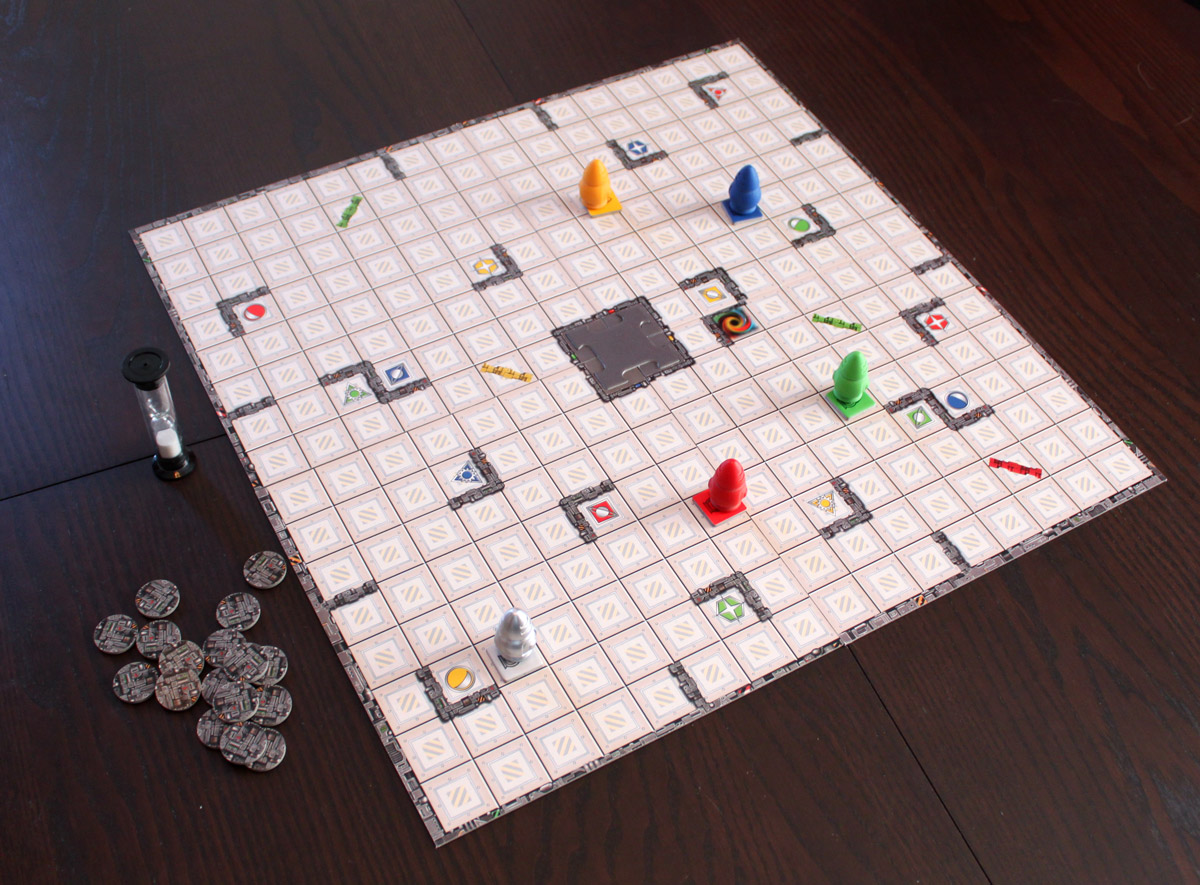
\includegraphics[scale=0.2]{imageRobot.jpg}
    \\[2cm]
    
 

    \begin{minipage}{0.4\textwidth}
      \begin{flushleft} \large
 { \color{RedViolet}\underline{Membres du groupe: }}\textsc{ } \
 \begin{enumerate}
 \item AIT KHEDDACHE Wissam
 \item BOUAOUD Malik
 \item SINI Lynda
 \item SI-MOHAMMED Sonia Taous
 \item CUQUEMELLE Mathieu
 \end{enumerate}
              \end{flushleft}
    \end{minipage}
    \begin{minipage}{0.4\textwidth}
      \begin{flushright} \large
\emph {\color{RedViolet}\underline{Enseignants: }} \\M.\textsc{BONNET Gregory}\\ M.\textsc{CHATEL Romain} \\ M.\textsc{SASSI Taoufik} 
     \\   \emph {\color{RedViolet}\underline{Groupe: }} \\  \textsc{4A \\ L2 Informatique}\\
      \end{flushright}
    \end{minipage}

    \vfill

    % Bottom of the page
    {\large 2019 / 2020 }

  \end{center}
  
 \end{titlepage}



\newpage

\tableofcontents
\setcounter{page}{0}

\newpage

\section{Introduction: }
La programmation orientée objet est un paradigme informatique que chaque informaticien doit maîtriser.
Ainsi, pour appliquer nos connaissances théoriques acquises tout au long de notre parcours académique, nous avons choisi de réaliser le projet de "Ricochet Robot Solver". Le but de ce projet est de développer un programme qui permet de trouver une solution optimale pour toute situation du jeu, c'est-à-dire trouver le plus court chemin entre deux objets.
Les parties principales du projet sont les suivantes: 
\begin{itemize}
\item Développement du moteur de jeu.
\item Implémentation d'un algorithme de résolution A*.
\item Implémentation des tables de transposition.
\item Réalisation d'une interface graphique avec JavaFx.
\end{itemize}


\section{Présentation du jeu :}
Ricochet Robot est un jeu de société sorti à l'origine en Allemagne sous le nom de Rasende Roboter. Il s'agit d'un jeu de parcours se jouant de un à plusieurs joueurs. Son objectif est d'atteindre une case objective en un minimum de déplacements possibles.

\subsection{Règles du jeu:}
\begin{itemize}
\item Assembler quatre sous-plateaux afin de construire le plateau du jeu.
\item Placer les quatre robots au hasard sur les cases du plateau.
\item Mélanger les jetons objectifs face cachée.
\item Retourner un jeton objectif: il indique la case objective et le robot qu'on doit bouger.
\item Trouver une solution pour atteindre la case cible en minimum de coups possibles, en respectant les règles de déplacement citées ci-dessous.
\end{itemize}

\subsection{Règles de déplacements:}
\begin{itemize}
\item Un robot se déplace horizontalement ou verticalement sans pouvoir s'arrêter jusqu'à ce qu'il rencontre un obstacle: bords du plateau, murs, plaque centrale, un autre robot.
\item Lorsqu'une barrière oblique colorée de la même couleur que le robot est rencontrée, le robot rebondit de 90\degree suivant la bonne direction.
\end{itemize}


\section{Organisation du projet}
\subsection{Modifications apportées sur les règles du jeu}
Les règles de ce jeu sont un peu compliquées à implémenter, et vu que nous sommes limités par le temps, nous nous sommes mis d'accord à faire certaines modifications sur le jeu.
\begin{enumerate}
\item Un obstacle est représenté par une case du plateau.
\item Un robot rencontré lors d'un déplacement est considéré comme un obstacle.
\item Un robot diffèrent du robot courant, ne peut être déplacé pour créer de nouveaux chemins.
\item L'assemblage aléatoire, et les rotations des plateaux, ne se font que du côté face. 
\end{enumerate}

\subsection{Répartition des tâches :}
Ce travail a été réalisé par tous les membres du groupe ,on a essayé de travailler sur toutes les parties qui composent le jeu .
\\
\begin{table}[h]
\begin{tabular}{|c|C{2cm}|C{2cm}|C{3cm}|c|C{2cm}|C{2cm}|c|}
\hline
Tâches &\multicolumn{2}{c|}{Construction du projet}&
  Implémentation de A* & \multicolumn{4}{c|}{interface graphique}\\
\hline
Participants & Construction du plateau & Mouvement des robots & A* & menu & plateau et son & mouvement des robots & rules \\
\hline
Malik & x & & x & & x & & \\ 
\hline
Wissam & x & & x & & & x & \\
\hline
Lynda & & x & x & & & & x \\
\hline
Sonia & & x & x & x & & & \\
\hline
Mathieu & x & x & & & & & \\
\hline
\end{tabular} 
\end{table}

\subsection{Architecture du code:}
\subsubsection{diagramme des packages:}
\begin{figure}[h]
\begin{center}
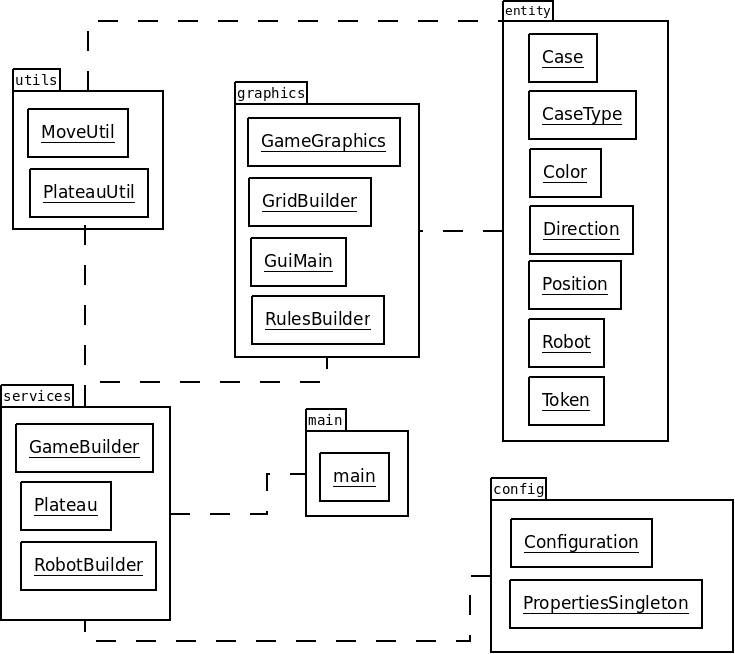
\includegraphics[scale=0.3]{DiagrammeDesPackages.png}
\end{center}
\end{figure}

Concernant l'architecture du projet, nous avons opté pour une décomposition en six packages : \\
\packagename{config}: Implémente le modèle de conception Singleton qui vise à contrôler l'initialisation des objets d'une classe particulière en garantissant qu'une seule instance de l'objet existe dans la machine virtuelle Java..\\
\packagename{entity} : Les entités nécessaires pour la construction de l'application .\\
\packagename{graphics}: La liaison entre le moteur du jeu et l'interface graphique\\
\packagename{main}: Classe test du jeu pour le lancer sur la console.\\
\packagename{services} : La couche métier qui correspond à la partie fonctionnelle de l'application.\\
\packagename{utils}: Il porte des classes utiles, comme la classes qui gère les mouvements des robots.\\

\subsubsection{Diagramme des classes: }
\begin{figure}[h]
\begin{center}
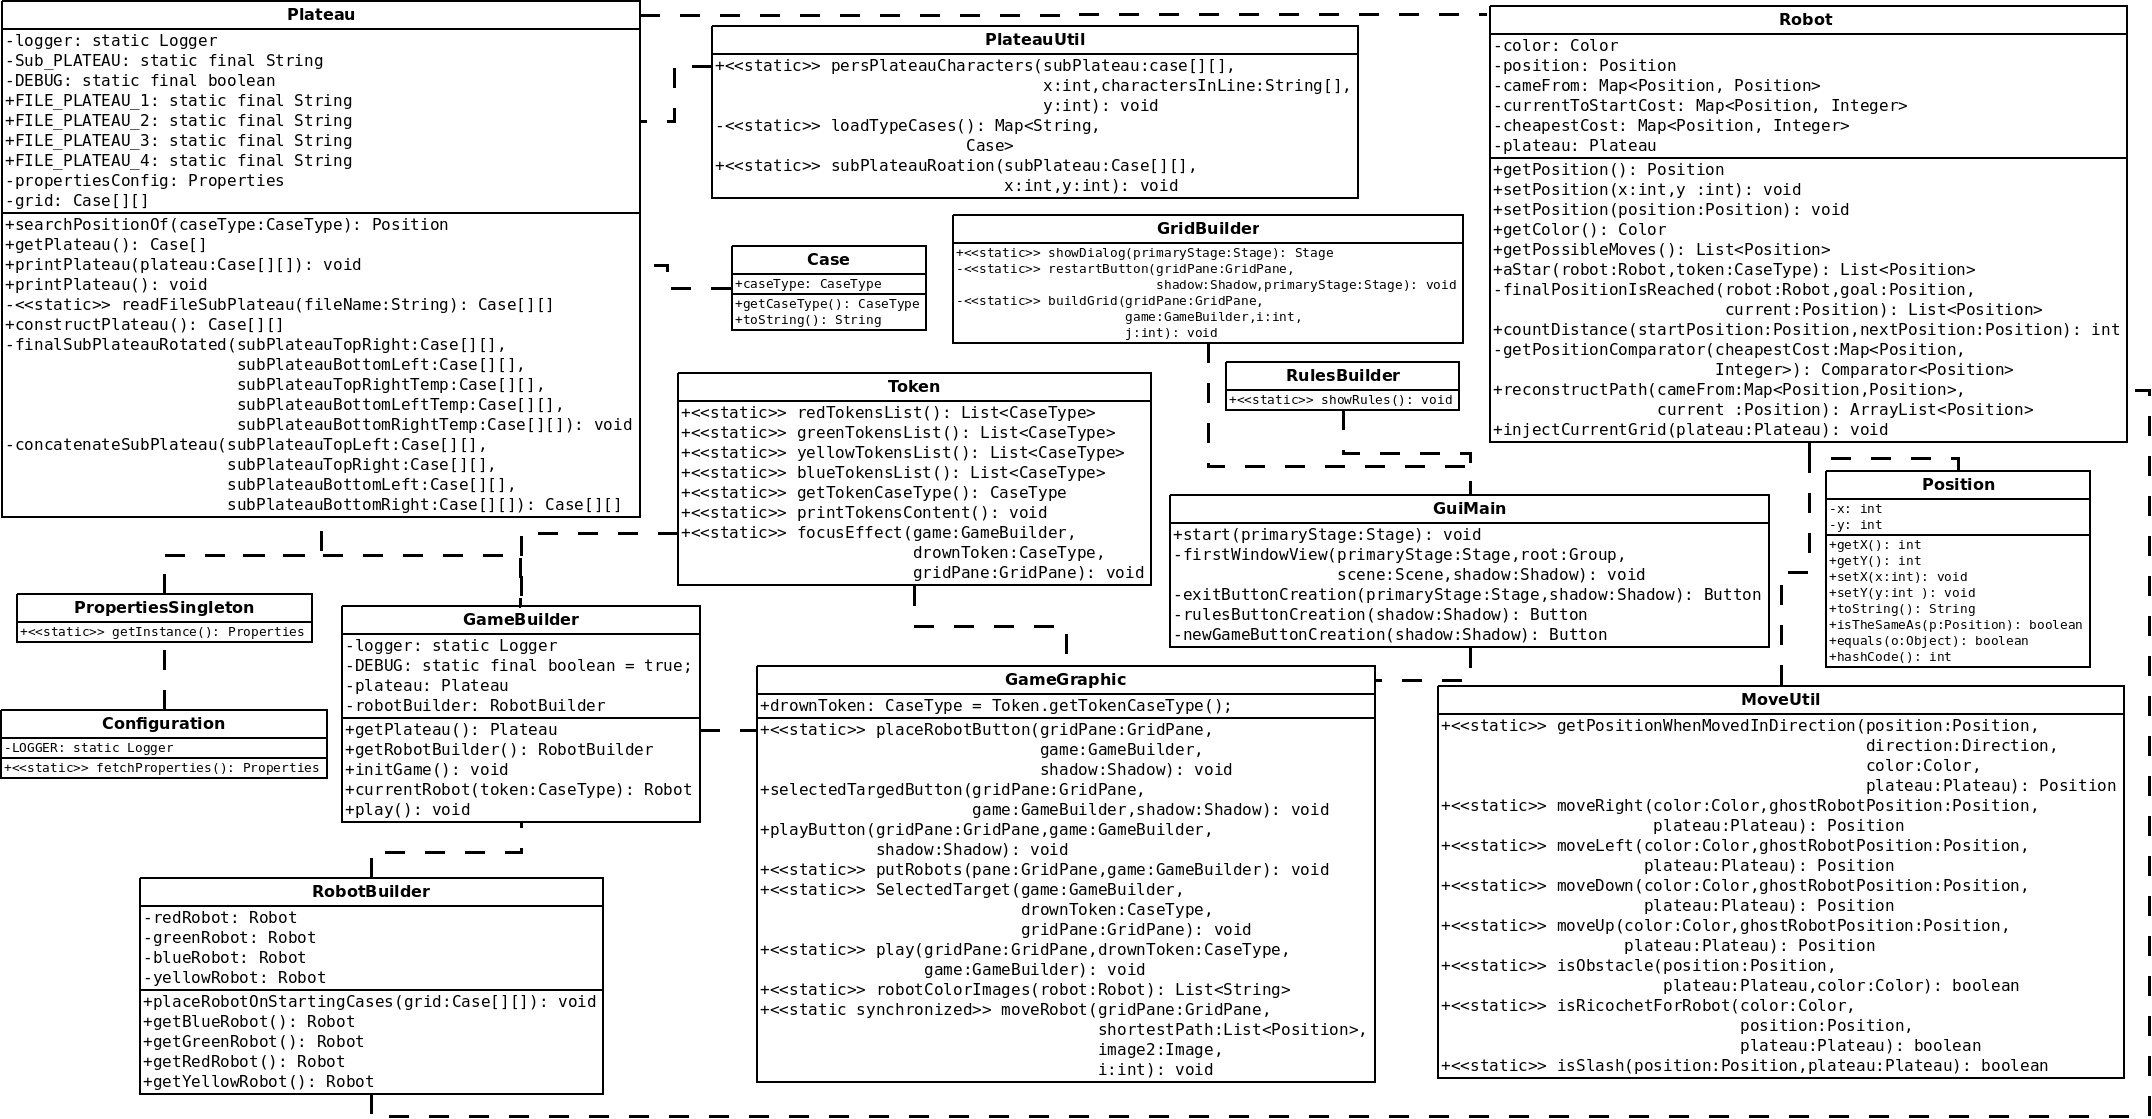
\includegraphics[scale=0.23]{DiagrammeDesClasses.png}
\end{center}
\end{figure}


\section{Éléments techniques:}
Les éléments techniques se reposent sur les 5 points cités ci-dessous, c'est-à-dire la lecture des fichiers pour générer les plateaux, l'algorithme de recherche A* amélioré grâce aux tables de transposition, l' interface graphique développée avec JavaFx et le design pattern Singleton.

\subsection{Lecture des fichiers:}
Les fichiers évoqués représentent les 4 sous plateaux formant le grand plateau du jeu. Nous avons tenu à garder impérativement cette caractéristique importante du jeu, c'est-à-dire le fait de pouvoir mélanger les 4 sous plateaux à chaque début de partie. Ce sont les classes \classname{Plateau} et \classname{PlateauUtil}, qui nous permettent de faire cet assemblage avec les méthodes suivantes:
\begin{itemize}
\item \methodename{readFileSubPlateau(Plateau)} : Consiste à la lecture d'un fichier (.txt) et retourne une matrice de case \textbf{case[][]}
\item \methodename{finalSubPlateauRotated(Plateau)} : Permet de réaliser la rotation des sous plateaux.
\item \methodename{subPlateauRotation (PlateauUtil)} : Réalise la rotation des éléments internes des sous plateaux .
\item \methodename{concatenateSubPlateau(Plateau)} : Concatène les 4 sous-plateaux 
\item \methodename{constructPlateau (Plateau)} : Consiste à lire les 4 sous plateaux et les assembler aléatoirement à l'aide des méthodes citées ci-dessus .
\end{itemize}
L'assemblage du plateau de jeu se fait donc dans la méthode \methodename{constructPlateau}, et se déroule comme ceci :
\begin{itemize}
\item On passe en paramètre un nom de fichier tiré aléatoirement avec la méthode \methodename{readFileSubPlateau}.
\item Appel à \methodename{finalSubPlateauRotated}, le côté haut-gauche reste inchangé, les autres font une rotation avec inversement des éléments internes de 90\degree (les ricochets) cet inversement concerne seulement le côté haut droit et bas-gauche. Le côté bas-droit fait une rotation de 180\degree , donc ses ricochets ne changent pas.
\item Après la réalisation de toutes ces opérations, il ne reste plus qu'à concaténer les 4 sous plateaux avec \methodename{concatenateSubPlateau}.
\end{itemize}

\subsection{Algorithme A*:}
\subsubsection{Présentation : }
A* est un algorithme qui consiste à trouver le plus court chemin entre un nœud initial et un nœud final dans un graphe, il est basé sur l’algorithme \textbf{Dijkstra}. A* a été créé pour que la première solution trouvée soit la meilleure. De plus cette extension est surtout une amélioration privilégiant la vitesse et la rapidité de calcul grâce à l'utilisation d'une \textbf{heuristique} d'évaluation, d'où sa célébrité dans le domaine de l'intelligence artificielle, plus précisément les jeux vidéo. Notre implémentation de l'algorithme a été perfectionnée pour rendre des résultats plus optimaux par rapport à l'original, et cela grâce à l'utilisation de l'heuristique adéquate, des tables de transposition, et le choix des différentes structures de données .


\subsection{Heuristique :}
Une heuristique dans le sens mathématique est un calcul fournissant rapidement une solution, pas nécessairement optimale ou exacte, à des fins d'optimisation.
Son utilisation dans A* consiste à évaluer la distance qui sépare chaque nœud visité du but à atteindre, et cela pour estimer le meilleur chemin, et explorer ensuite les nœuds restants par rapport à cette évaluation.
Mais il existe plusieurs façons pour calculer une heuristique, et donc le choix de cette dernière repose sur le fait de ne pas surestimer la distance du point de départ vers le point d'arrivée, et c'est son utilisation qui distingue A* des autres algorithmes existants.
Comme notre jeu impose 4 directions possibles de mouvements aux robots, nous utiliserons donc : une taxi-distance alias \textit{distance de Manhattan}.


\subsection{Implémentation :}
\LinesNumberedHidden
\DontPrintSemicolon
\begin{algorithm}[H]
\begin{tcolorbox}
\caption{\sc Algorithme A*}
\SetAlgoLined
\KwIn{Robot robot, CaseType token}
\KwOut{Une Liste de Positions }
\textbf{Variables : }\\  tentativeGscore : entier\\ startPosition, targetPosition, nextMove, current : Position \\ cheapestCost, currentToStartCost :  Map<Position, Integer> \\  finalSmallestPath, possibleMoves : List<Position> \\  cameFrom : Map<Position, Position> \\
 comparator : Comparator<Position>\\  openQueuePositions : Priorityqueue<Position>\\  openSetPositions : Set<Position>\\
\Begin{
$startPosition \gets new Position(robot.getPosition().getX(),robot.getPosition().getY())$\;
$targetPosition \gets plateau.searchPositionOf(token)$\;
$comparator \gets getPositionComparator(cheapestCost)$\;
$openQueuePositions \gets new PriorityQueue<>(1,comparator)$\;
$openSetPositions \gets new HashSet<>()$\;
$openQueuePositions.add(startPosition)$\;
$openSetPositions.add(startPositions)$\;
$gScore.put(startPosition,0)$\;
$fScore.put(startPosition,countDistance(startPosition,targetPosition))$\;
\While{$!openQueuePositions.isEmpty()$} {
$current \gets openQueuePositions.poll()$\;
$openSetPositions.remove(current)$\;
$gScore.put(current,countDistance(startPosition,current))$\;
$finalSmallestPath \gets finalPositionIsReached(robot,targetPosition,current))$\;
\If{$§finalSmallestPath.isEmpty()$}{ \Return finalSmallestPath;}
$robot.setPosition(current)$\;
$possibleMoves \gets getPossibleMoves()$\;
\For{$nextMove \in possibleMoves $}{
$tentativeGscore \gets gScore.getOrDefault(current$\;
$,Integer.MAX\_VALUE) +15$\;
\If{$tentativeGscore < currentToStartCost.getOrDefault(nextMove,$\;
$Integer.Max\_VALUE))$}{
$cameFrom.put(nextMove, current)$\;
$fScore.put(nextMove, tentativeGscore$\; $+ countDistance(nextMove, targetPosition))$\;
\If{$!openSetPositions.contains(nextMove)$}{
$openQueuePositions.add(nextMove)$\;
$openSetPositions.add(nextMove)$\;}}}}
\Return {Collections.emptyList()}\;}
\end{tcolorbox}
\end{algorithm}

\subsubsection{Déroulement :}
Après l'initialisation des structures de données, nous ajoutons au gScore, et fScore la position initiale du robot, avec comme  valeur 0 pour le gScore, et la valeur de la Map fScore.
\begin{equation}(valeur) fScore=gScore+heuristique\end{equation}
Initialement openQueuePosition est non vide, donc nous récupérons une position avec la méthode \methodename{poll} (ayant le fScore le plus intéressant).
On ajoute à la Map gScore la position et la distance entre le point de départ et le point courant.
\\Ensuite, on appelle la méthode \methodename{finalPositionIsReached} ,qui retourne une liste de positions, si une liste non vide est retournée cela signifie que l'objectif a été atteint, et qu'on doit arrêter de faire tourner notre algorithme.
\\Sinon(cas de la liste vide) le robot se place dans la case courante, et on appelle la méthode \methodename{getpossiblemoves}.
\\Après cela tentativeGscore reçoit soit, le score du noeud, s'il a été visité, sinon: \begin{equation} tentativeGscore=+\infty +N (N>=15) \end{equation}
\\ Dans le pseudoCode de A*, N vaut exactement 1 ,mais comme nos robots n'explorent pas forcément leurs cases voisines, nous avons remplacé ce $1$ qui génère des boucles infinis par $N>=15$ pour faire "grossir" artificiellement tentativeGscore, car à l'origine A* cherchera à minimiser le nombre de coups vers une destination.
\\Si tentativeGscore < gScore, donc ce nœud est plus intéressant que tous les nœuds précédemment visités, car son coût est inférieur, cameFrom représente une map ayant comme clé la position suivante à celle de la valeur, en d'autres termes, chaque position a comme clé sa position suivante.
\\On ajoute le nœud satisfaisant la condition précédente dans la map, et on enregistre son fScore dans sa Map, si le nœud nextMove n'est pas dans le set donc il n'est pas aussi dans la priorityQueue donc il n'a pas été visité, on doit alors l'enregistrer.
Cette boucle continue à tourner tant que \methodename{finalpositionIsReached} ne nous retourne pas de liste vide, dans le cas échéant la méthode ne retourne jamais de liste non vide ce qui signifie donc qu'il n'y a pas de solution pour atteindre le jeton cible.\\
\textbf{Pseudo-code de \methodename{finalpositionIsReached} :}

\LinesNumberedHidden
\DontPrintSemicolon
\begin{algorithm}[H]
\begin{tcolorbox}
\caption{\sc finalpositionIsReached }
\SetAlgoLined
\KwIn{Robot robot, Position goal, Position current}
\KwOut{Une Liste de Positions }
\textbf{Variables : }\\ aStarArray : ArrayList<Position> \\  cameFrom : Map<Position, Position> \\
\Begin{
\If{$((current.getX() == goal.getX()) \textbf{et} (current.getY() == goal.getY()))$}{
$aStarArray \gets reconstructPath(cameFrom, current)$\;
$robot.setPosition(aStarArray.get(aStarArray.siz() - 1)$\;
\Return aStarArray;}
\Return {Collections.emptyList()}\;}
\end{tcolorbox}
\end{algorithm}

\methodename{finalPositionIsReached} à l'aide de la Map cameFrom qui contient comme \textbf{clé} la position \underline{suivante} de celle de la \textbf{valeur},nous retourne une ArrayList de positions contenant le chemin à prendre depuis le départ vers l'arrivée.


\subsubsection{Tables de transposition}
Une table de transposition est un cache de positions précédemment vues et d'évaluations associées, dans une arborescence de jeux générée par un programme de jeu informatique, voici une illustration meilleur ci-dessous (figure \ref{fig:Table De Transposition}) :
\begin{figure}[H]
\begin{center}
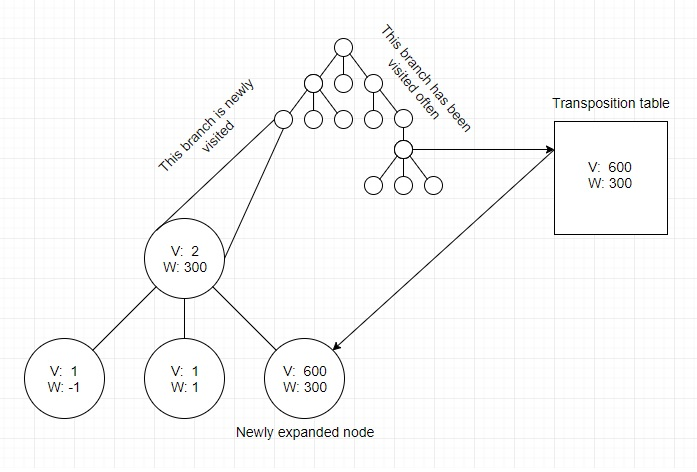
\includegraphics[scale=0.25]{transpo.jpg}
\\[1cm]
\end{center}
\caption{Graphe d'une table de transposition}
\label {fig:Table De Transposition}
\end{figure}
Notre implementation de l'algorithme A*,  repose sur l'utilisation des tables de transposition, c'est le sens des HashMap \textbf{gScore} et \textbf{fScore}. Elles sont utilisées pour ne pas ré-étendre les nœuds ayant été déjà visités, ou un nœud avec un fScore inférieur à ce qui a déjà été trouvé, et donc A* gagne en rapidité considérablement.


\subsubsection{La complexité}
La complexité de A* dépend de l'heuristique utilisée, dans notre cas c'est \textit{la distance de Manhattan}, elle est dans le pire des cas égale à celle de Dijkstra une complexité exponentielle \textbf{{O}$(e^n)$} où n est le nombre de nœuds du graphe, on rappelle qu'on a utilisé un Set au lieu de faire \textit{priorityQueue.contains} et cela  diminue la complexité de cette vérification qui passe de \textbf{{O}$(\log(n))$} à \textbf{{O}(1)}.

\subsection{Design pattern Singleton}
Un modèle de conception décrit une solution établie aux problèmes les plus fréquemment rencontrés dans la conception de logiciels.
Le pattern Singleton vise à garder un contrôle sur l'initialisation d'une classe, en veillant à ce qu’une seule instance de l’objet existe dans toute la machine virtuelle Java.
C'est ce qu'on a fait dans le package \packagename{config}, qui assure qu'une seule instance de classe Properties soit crée.
Tout d'abord on crée une variable statique qui va permettre de stocker l'unique instance de la classe, c'est l'équivalent de l'attribut static "instance" crée dans la classe \classname{PropertiesSingleton}, Si celui-ci est nul alors on crée une instance de la classe et on stocke sa valeur dans cet attribut. Sinon c’est que l’attribut possède déjà une instance de la classe. Dans tous les cas la méthode retourne la valeur de l’attribut possédant l’unique instance de la classe.
Dans notre implémentation, nous avons créé une classe interne statique \classname{SingletonHolder}, qui détient l’exemple de la classe Singleton. Il ne crée l’instance que si un appelle à  la méthode \methodename{getInstance()} advient ,et non pas lorsque la classe extérieure est chargée.
En outre, il faut noter que le constructeur a le modificateur d’accès privé. Il s’agit d’une exigence pour créer un Singleton, car un constructeur public signifierait que n’importe qui pourrait y accéder et commencer à créer de nouvelles instances.

\subsection{Interface graphique avec Java Fx}
JavaFx offre des interfaces graphique plus élégante que celle du swing , c'est pour cela qu'on l'a choisi pour l’implémentation graphique.
le paquet \textit{graphics} contient toutes nos méthodes implémentant une interface graphique. Nous avons 3 classes : 
\begin{itemize}
\item \classname{GridBuilder} : Contient des méthodes \methodename{showDialog, buildGrid, restartButton} créant un GridPane représentant notre plateau du jeu.
\item \classname{RuleBuilder} : Contient une méthode \methodename{showRules} affichant les règles du jeu. 
\item \classname{GameGraphic} : Abrite plusieurs méthodes faisant marcher le jeu après l'affichage de la grille :
	\begin{itemize}
	\item[\textbullet] \methodename{placeRobotButton} charge les images des robots dans la grille grâce à un bouton. 
	\item[\textbullet] \methodename{selectedTargetButton} crée un bouton qui ajoute un effet lumineux sur le jeton courant grâce au filtre RGB utilisé par la méthode \methodename{focusOnSelectedTarget}.
	\item[\textbullet] \methodename{playButton} crée un bouton "play"  faisant appel à la méthode \methodename{play()} qui retrace le parcours du robot. 
	\end {itemize}
\item \classname{GuiMain} : Affiche la présentation du jeu (le Menu du jeu) avec 3 bottons : New Game, Rules, Exit.
	\begin{itemize}
	\item[\textbullet] New Game : Pour commencer la partie.
	\item[\textbullet] Rules : Pour afficher les règles de jeu. 
	\item[\textbullet] Exit : Pour quitter le jeu.
	\end {itemize}
\end{itemize}
\textbf{\underline{Remarque :}}Musique enclenchée au lancement du jeu ,et tous les boutons ont un effet shadow d'animation  lorsque la souris pointe sur un d'entre eux .

\subsection{Utilisation de l'application:}
Le jeu est un projet gradle. Gradle est un système de build qui permet de construire un projet java (structure et héirarchie).
\subsubsection{Lignes de commandes :}
Voici quelques commandes à lancer afin d'éxécuter le projet : \\Placez vous dans le dossier robot-ricochet-mc-mb-wa-ls-ss (cf README).
\begin{itemize}
 \item Sous Linux:
	\begin{itemize}
	\item \textit{./gradlew build}: génération du dossier build qui contient des sous dossiers contenant les binaires ...(les outputs).
 	 \item \textit{ ./gradelew run}: lancer le jeu .
 	\item \textit{ ./gradelew javadoc} : génération d'un dossier docs/javadoc dans build qui contient la javadoc du projet.
  	\item \textit{./gradelew jar}: génération du jar exécutable dans build/libs.
 	\item \textit{ ./gradelew clean}: supprimer le dossier build.
	\end{itemize}
 \item Sous Windows:  Pour lancer le jeu il suffit de lancer la commande \textit{gradle.bat run}.
 \item Sous MacOs: Les mêmes commandes que linux mais au lieu de mettre \textit{./gradlew run} (exemple) il suffit de mettre \textit{gradle run}.
\end{itemize}
\newpage
\subsubsection{Utilisation de l'interface graphique:}
Après le lancement du  programme, vous obtenez la figure \ref{fig:Menu} ci-dessous, qui représente le Menu du jeu :
\begin{figure}[H]
\begin{center}
 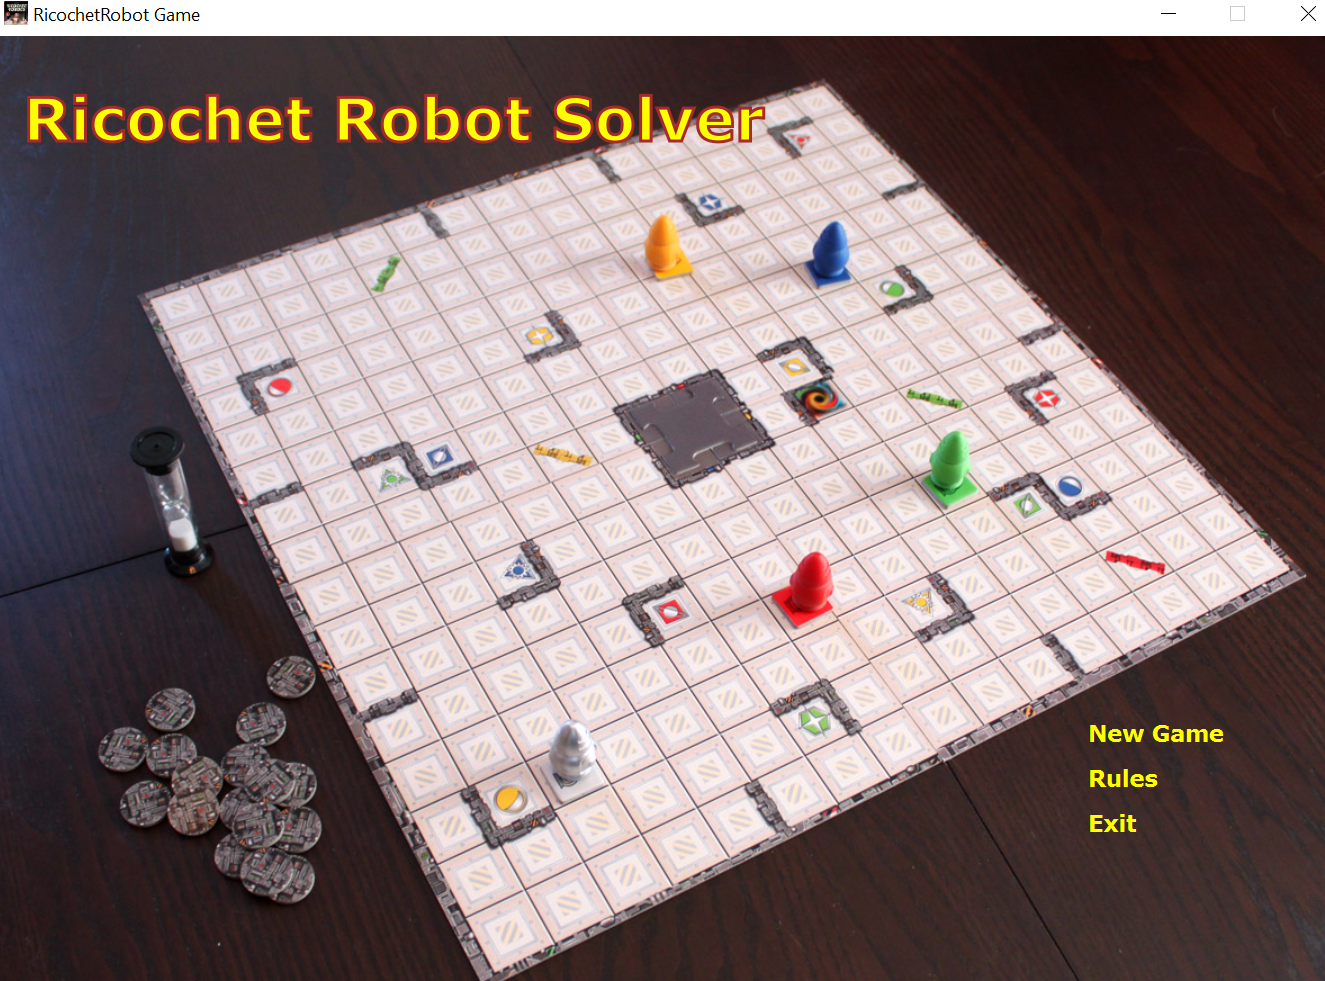
\includegraphics[scale=0.4]{Screen1.png}
    \\[1cm] 
\end{center}  
\caption{Menu du Jeu} 
\label{fig:Menu}
\end{figure}

Si vous cliquez sur le bouton \textbf{NewGame} vous obtiendrez la figure \ref{fig:Jeu} :\\
\begin{figure}[H]
\begin{center}
 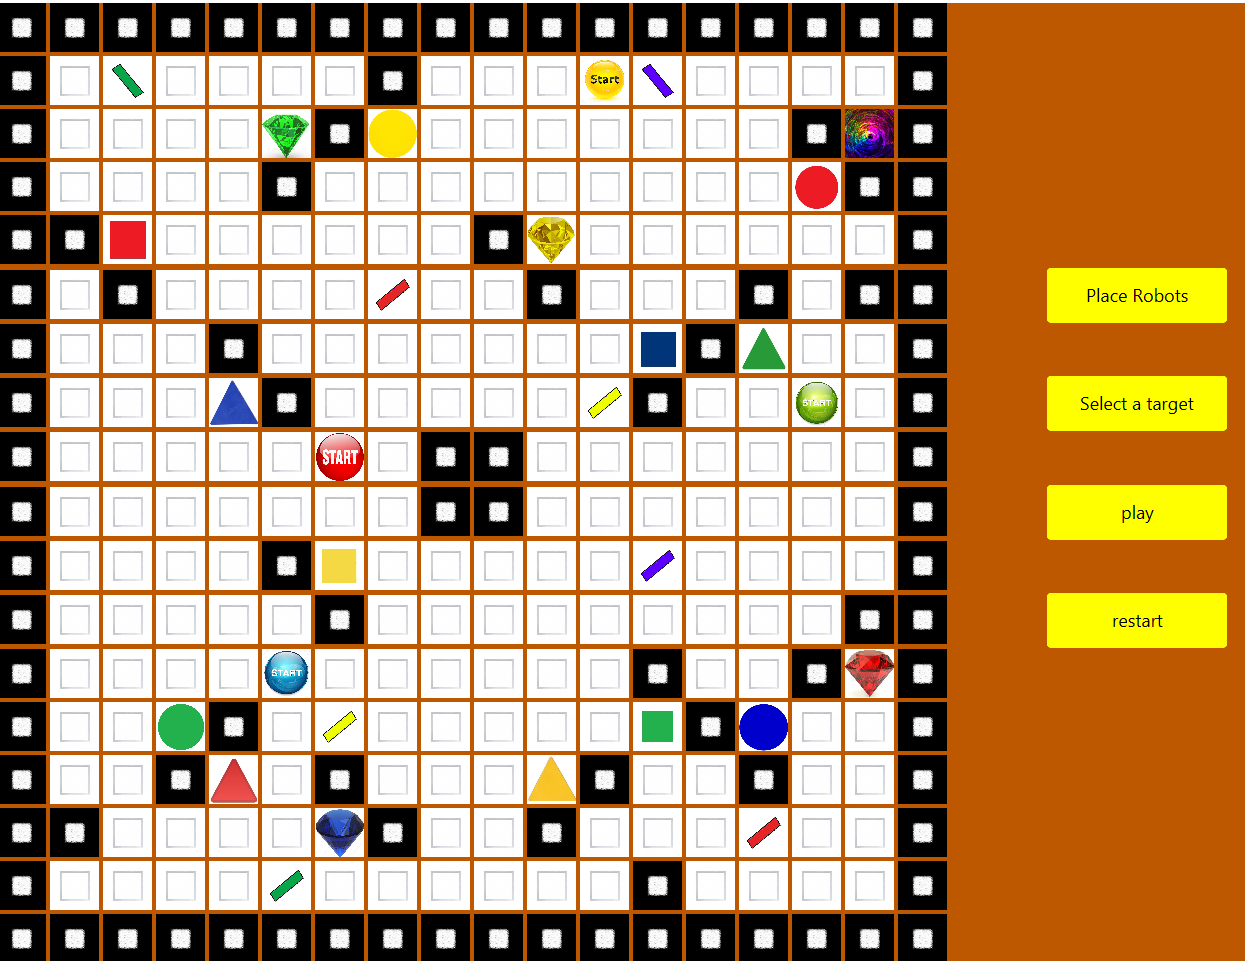
\includegraphics[scale=0.4]{Screen2.png}
    \\[1cm]     
   
\end{center}  
\caption{Lancement du Jeu}
\label{fig:Jeu}  
\end{figure}

Vous pouvez jouez en cliquant successivement sur les boutons suivants : \textbf{Place Robots} --> \textbf{Select a target } --> \textbf{Play}.
\\Le bouton \textbf{Restart} c'est pour rejouer.\\
Et si vous cliquer sur \textbf{Rules}, vous provoquez l'affichage de cette fenêtre (figure \ref{fig:Rules}), qui explique les règles du jeu implémentés. 
\begin{figure}[H]
\begin{center}
 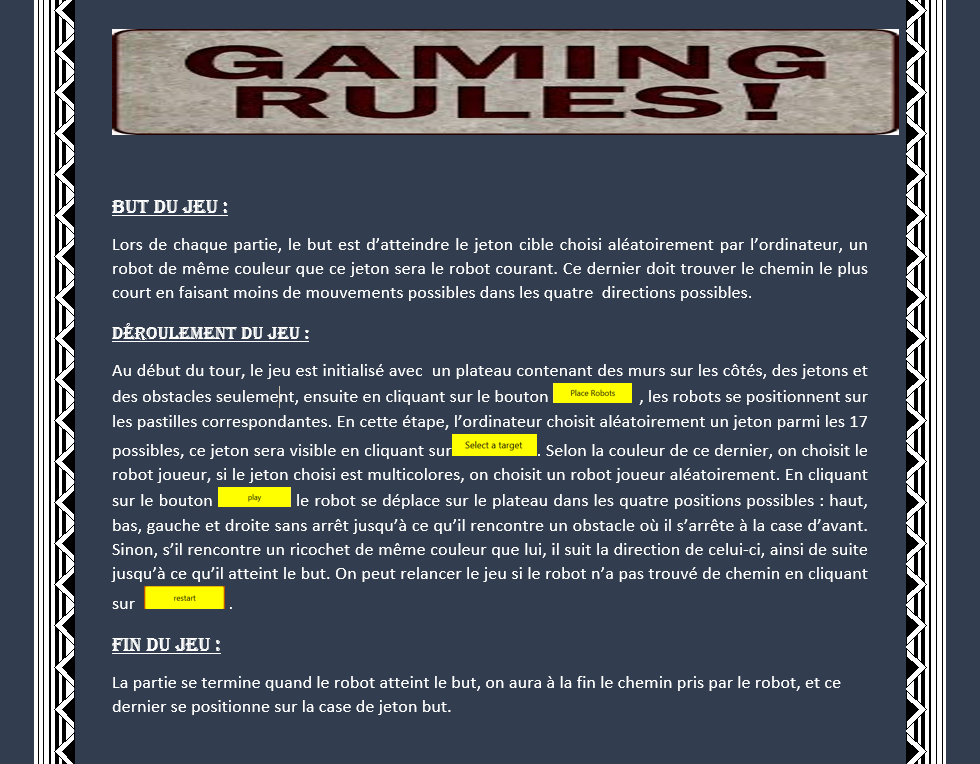
\includegraphics[scale=0.5]{rules.png}
    \\[1cm] 
       
\end{center}  
\caption{Règles du jeu } 
\label{fig:Rules}
\end{figure}



\section{Conclusion}
\subsection{Objectifs remplis}
A terme de ce rapport, qui présente les détails d’un projet qu’on a réalisé en groupe de cinq étudiants, nous sommes arrivés à implémenter et optimiser  l’algorithme d’intelligence artificielle \textbf{A*} qui cherche le plus court chemin qu'un robot peut emprunter pour atteindre l'objectif.
\par
Ce travail nous a permis d’enrichir nos connaissances en informatique et précisément en Java, on a appris à  utiliser \textbf{Git, Gradle, JavaFx}, on a réussi à implémenter un algorithme difficile comme \textbf{A*}, ainsi que l’application des bases acquises en cours.
\par
Le travail d’équipe, la répartition équitables des tâches, la bonne gestion de temps et le partage d’idées nous a apporté une bonne expérience dans le déroulement de ce projet  .

\subsection{Améliorations possibles}
Pour conclure on pourrait apporter des modifications sur ce projet, par exemple, dans la construction du plateau on pourrait utiliser des murs autour des cases pour représenter les obstacles au lieu de représenter une case entière comme obstacle, ceci nous permettra d’avoir moins de blocage lors de la recherche du chemin .
\par
Concernant les règles du jeu, nous pourrions également ne pas considérer les autres robots différents du robot courant comme des obstacles fixes, mais dynamiques, c'est à dire déplaçable de sorte que A* trouve d'autres chemins si la situation est bloquée, aussi l'utilisation d'une autre formule que la distance de Manhattan pour calculer l’heuristique
\par
Finalement, concernant l'interface graphique elle pourrait être plus animée,  par exemple création d'un effet graphique indiquant que le robot a gagné le tour,ou bien un effet sonore des applaudissements ... 

\newpage
\begin{thebibliography}{1}
\bibitem{notes} wikepedia [en ligne] Disponible sur  \\\texttt{https://en.wikipedia.org/wiki/A*-search-algorithm}.
\bibitem{notes} openclassrooms [en ligne] Disponible sur  \\\texttt{https://openclassrooms.com/fr/courses/26832-apprenez-a-programmer-en-java/5014486-decouvrez-java-fx}.
\bibitem{notes}  Stackoverflow [en ligne] Disponible sur  \\\texttt{https://stackoverflow.com/questions/2049380/reading-a-text-file-in-java}.
\bibitem{notes}  Developpez.com [en ligne] Disponible sur  \\\texttt{ https://mikarber.developpez.com/tutoriels/java/introduction-javafx}.
\bibitem{notes} Codeflow [en ligne] Disponible sur  \\\texttt{ https://www.codeflow.site/fr/article/gradle}.
\bibitem{notes} Gimps [logiciel du dessin] téléchargeable sur \\\texttt{https://www.gimp.org/downloads/}.
\bibitem{notes} Google images [en ligne] Disponible sur \\\texttt{ https://www.google.com/}.
\bibitem{notes} Heuristics From Amit’s Thoughts on Pathfinding [en ligne] Disponible sur  \\\texttt{https://theory.stanford.edu/~amitp/GameProgramming/Heuristics.html}.
\bibitem{notes} Baeldung [en ligne] Disponible sur \\\texttt{ https://www.baeldung.com/creational-design-patterns}.
\end{thebibliography}

\end{document}